\documentclass{beamer}
\usetheme{Dresden}
\usecolortheme{orchid}

\usepackage[french]{babel}
\usepackage[utf8]{inputenc}
\usepackage[T1]{fontenc}
\usepackage{graphicx}
\usepackage{tikz}
\usepackage{fontawesome}
\usepackage{amsmath}
\usepackage{algorithm}
\usepackage{algpseudocode}

\graphicspath{{../report/ims/}{ims/}}

\newcommand{\N}{\mathbb{N}}

\title{Vérification de la perspective dans les peintures}
\subtitle{Stage de M1}
\date{4 Septembre 2019}
\author{
	Yoann Coudert--Osmont \inst{1} \newline
	\textit{Encadré par} Elmar Eisemann \textit{et} Ricardo Marroqium \inst{2}
}
\institute{
	\inst{1} ENS de Lyon \and
	\inst{2} TU Delft
}

\begin{document}
	
	\begin{frame}
		\titlepage
	\end{frame}

	\section{Règles de perspective}

	\begin{frame}{Lignes et points de fuites}
		\centering
		\begin{figure}
			\begin{tikzpicture}[thick, scale=1.2]
			\draw[] (0, 0) -- (1, 0) -- (1, 1) -- (0, 1) -- cycle;
			\draw[red] (-2.5, 2.25) -- (6, 2.25);
			\draw[green] (0, 1) -- (0.8, 1.5);
			\draw[green, dashed] (0.8, 1.5) -- (2, 2.25);
			\draw[green] (1, 1) -- (1.4, 1.5);
			\draw[green, dashed] (1.4, 1.5) -- (2, 2.25);
			\draw (0.8, 1.5) -- (1.4, 1.5);
			\draw[green] (1, 0) -- (1.4, 0.9);
			\draw[green, dashed] (1.4, 0.9) -- (2, 2.25);
			\draw (1.4, 0.9) -- (1.4, 1.5);
			
			\node[blue] (VP) at (2, 2.25) {$\bullet$};
			\node[above, blue] at (2, 2.25) {\small Point de fuite};
			\node[below, red] at (5, 2.25) {\small Ligne de fuite};
			\node[left, green] at (0.4, 1.4) {\small Lignes parallèles};
			\end{tikzpicture}
		\end{figure}
	\end{frame}

	\begin{frame}
		\centering
		\begin{figure}[h]
			\begin{tikzpicture}[thick, yscale=0.65, xscale=0.82]
			\draw[very thick] (0, 6) -- (12, 6);
			\draw[semithick] (0, 0) -- (12, 0);
			\node[above] at (6, 6) {\small Ligne de fuite};
			\node[above, red] at (0, 6) {\small $A$};
			\node[above, blue] at (4, 6) {\small $B$};
			\node[above, green] at (12, 6) {\small $C$};
			
			\foreach \i in {2, ..., 11} \draw[red] (0, 6) -- (\i, 0);
			\foreach \i in {1.333, 2.666, ..., 9.333} \draw[blue] (4, 6) -- (\i, 0);
			
			\draw[red] (2, -0.3) node {\texttt{|}} -- node[below] {$d_A$} (3, -0.3) node {\texttt{|}};
			\draw[blue] (4, -0.3) node {\texttt{|}} -- node[below] {$d_B$} (5.333, -0.3) node {\texttt{|}};
			\draw[green] (6, -0.3) node {\texttt{|}} -- node[below] {$d_C$} (8, -0.3) node {\texttt{|}};
			
			\node[below, align=center] at (10.2, 0)
			{\footnotesize ligne parallèle à \\[-1mm]
				\footnotesize la ligne de fuite};
			
			\clip (0, 0) rectangle (12, 6);
			\foreach \i in {-4, -2, ..., 10} \draw[green] (12, 6) -- (\i, 0);
			\foreach \i in {4, 8, ..., 24} \draw[blue] (-12, 6) -- (\i, 0);
			\end{tikzpicture}
		\end{figure}
		$$ {\color{blue} B} = \dfrac{{\color{green} d_C} {\color{red} A} + {\color{red} d_A} {\color{green} C}}{{\color{red} d_A} + {\color{green} d_C}} \qquad {\color{blue} d_B} = 2 \dfrac{{\color{red} d_A} {\color{green} d_C}}{{\color{red} d_A} + {\color{green} d_C}} $$
	\end{frame}

	\section{Détection des lignes}
	
	\begin{frame}{Les étapes}
		\begin{itemize}
			\small \item Changement d'espace de couleurs (RGB $\rightarrow$ CIE Lab)
			\small \item Lissage / élimination du bruit
			\small \item Calcul du gradient
			\small \item Transformée de Hough
			\small \item Regroupement des lignes et calcul des points de fuites
		\end{itemize}
		\centering
		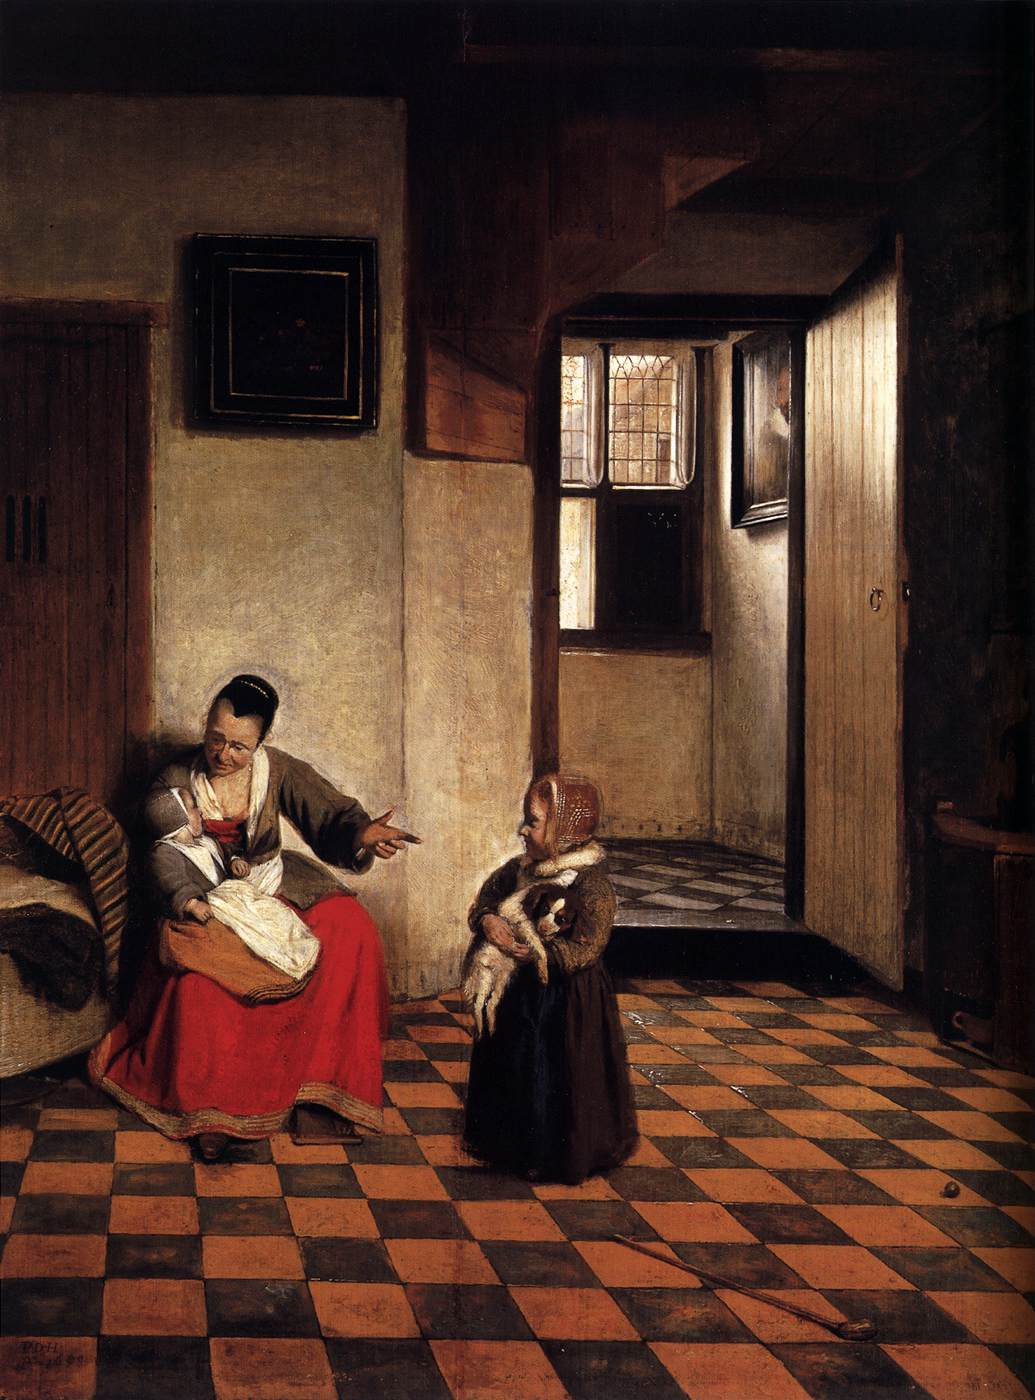
\includegraphics[scale=0.33]{hooch1.jpg}
		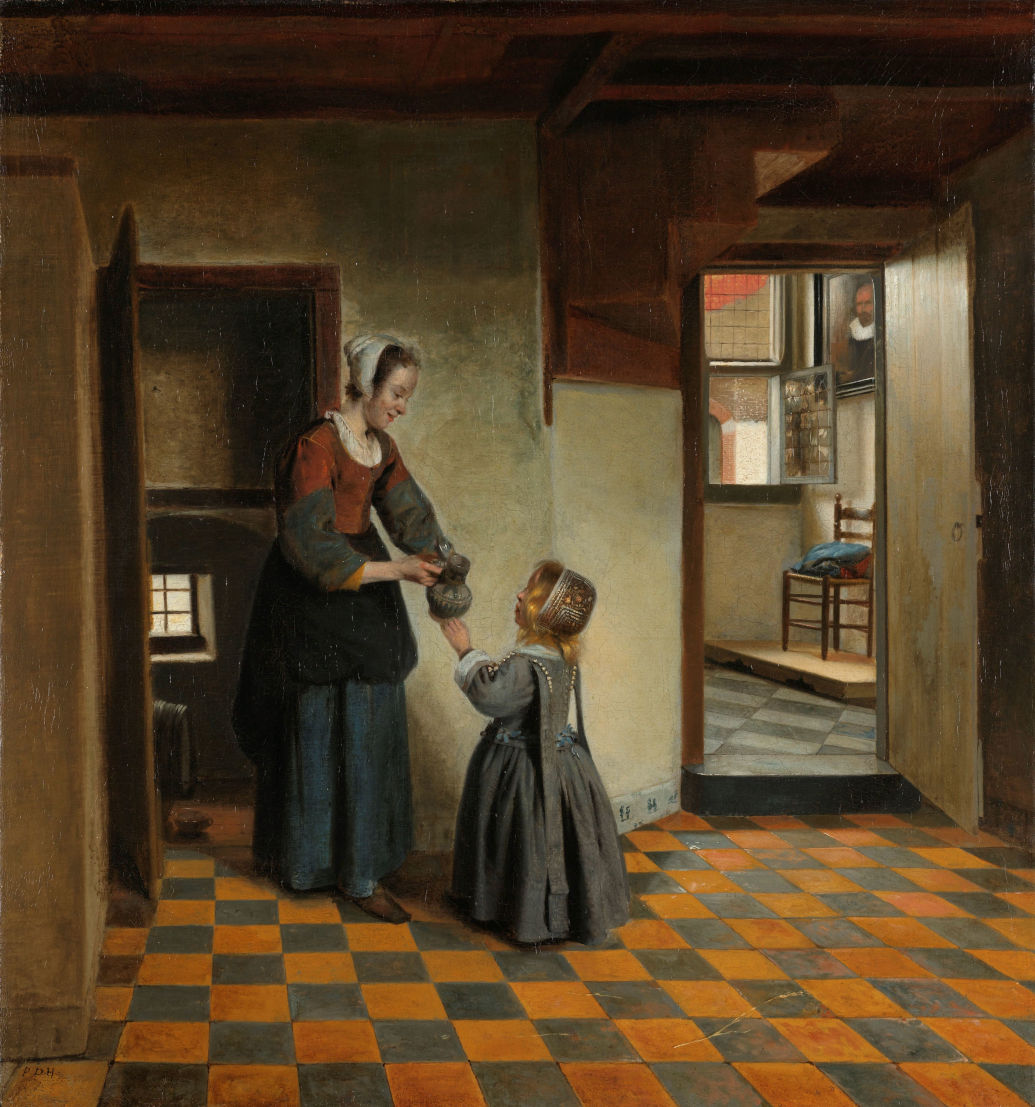
\includegraphics[scale=0.4]{hooch2.jpg}
	\end{frame}

	\begin{frame}{CIE Lab}
		Besoin d'un espace dans lequel la distance entre deux couleur est en accord avec l'œil humain :
		$$ \Delta E = \sqrt{(R_1 - R_2)^2 + (V_1 - V_2)^2 + (B_1 - B_2)^2} \qquad \text{\huge \color{red} \text{\faThumbsODown}} $$
		$$ \Delta E = \sqrt{(L_1^* - L_2^*)^2 + (a_1^* - a_2^*)^2 + (b_1^* - b_2^*)^2} \qquad \text{\huge \color{green} \text{\faThumbsOUp}}  $$
	\end{frame}

	\begin{frame}{Filtre gaussien}
		\centering
		\begin{tikzpicture}[scale=0.8]
		\node at (0, 0.9) {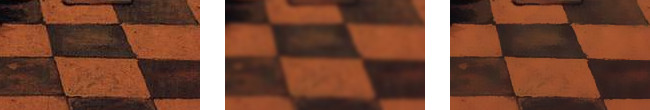
\includegraphics[width=8cm]{smoothing.jpg}};
		\node[below] at (0, 0) {\small Filtre gaussien};
		\node[below] at (-3.45, 0) {\small Image original};
		\fill[white] (1.7, 0) rectangle (5.1, 2);
		\fill[white] (-5.1, 0) rectangle (-8.6, 2);
		\end{tikzpicture}
		$$ I'(z) = \dfrac{1}{W} \sum_{z' \in \Omega_{z}} I(z') \exp \left( - \dfrac{\| z - z'\|^2}{2 \sigma^2} \right) $$
		\small Où $\Omega_{z}$ est une fenêtre autour de $z \in \N^2$ et $W = \sum_{z' \in \Omega_{z}} \exp \left( - \frac{\| z - z'\|^2}{2 \sigma^2} \right)$.
	\end{frame}

	\begin{frame}{Filtre bilatéral}
		\centering
		\begin{tikzpicture}[scale=0.8]
		\node at (0, 0.9) {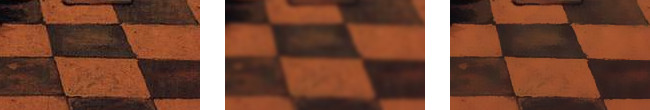
\includegraphics[width=8cm]{smoothing.jpg}};
		\node[below] at (0, 0) {\small Filtre gaussien};
		\node[below] at (-3.45, 0) {\small Image original};
		\node[below] at (3.45, 0) {\small Filtre Bilatéral};
		\end{tikzpicture}
		$$ I'(z) = \dfrac{1}{W} \sum_{z' \in \Omega_{z}} I(z) \, f(z, z') \, g \left( I(z), I(z') \right) $$
		\small Où $\Omega_{z}$ est une fenêtre autour de $z$ et $W = \sum_{z' \in \Omega_{z}} f(z, z') g(I(z), I(z'))$.
		$$ f(z, z') = \exp \left( - \dfrac{\| z - z'\|^2}{2 \sigma_f^2} \right) \qquad g(u, u') = \exp \left( - \dfrac{\| u - u'\|^2}{2 \sigma_g^2} \right) $$
	\end{frame}

	\begin{frame}{Sélection de zone intéressante}
		\begin{figure}[h]
			\centering
			\begin{tikzpicture}[scale=0.75]
			\node (a) at (0, 0) {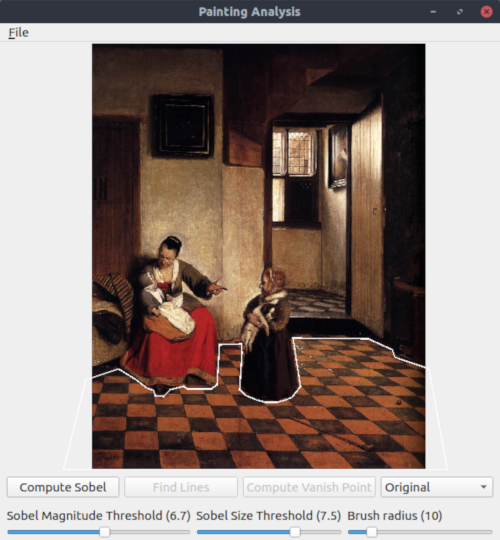
\includegraphics[scale=0.75]{zone_select.png}};
			\node (b) at (8.5, 0) {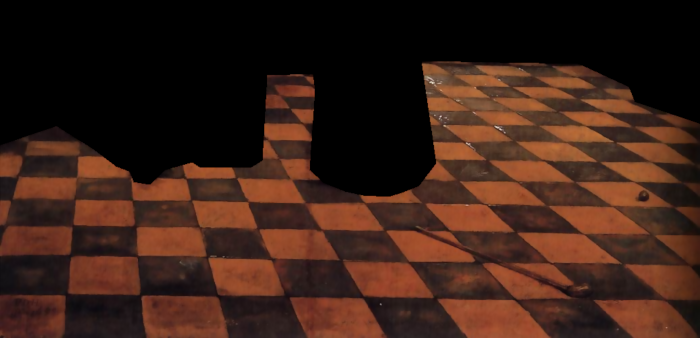
\includegraphics[scale=0.9]{bilateral.png}};
			\draw[->, ultra thick] (a) -- node[above, align=center]
			{\footnotesize Coupe et \\[-1mm]
				\footnotesize application du \\[-1mm]
				\footnotesize filtre bilatéral} (b);
			\end{tikzpicture}
		\end{figure}
	\end{frame}

	\begin{frame}{Gradient (filtre de Sobel)}
		$$ G_{C, x} = \begin{bmatrix} -3 & 0 & 3 \\ -10 & 0 & 10 \\ -3 & 0 & 3 \end{bmatrix} \ast C
		\qquad G_{C, y} = \begin{bmatrix} -3 & -10 & -3 \\ 0 & 0 & 0 \\ 3 & 10 & 3 \end{bmatrix} \ast C
		$$
		$$ G_C = \sqrt{G_{C, x}^2 + G_{C, y}^2} $$
		\begin{block}{Amplitude du gradient}
			\vspace{-2mm}
			$$ G = \sqrt{G_{L^*} + G_{a^*} + G_{b^*}} $$
		\end{block}
	\end{frame}

	\begin{frame}{Gradient (filtre de Sobel)}
		On définie $(G_{C, x}', \, G_{C, y}')$ égal à $(G_{C, x}, \, G_{C, y})$ si $G_{C, x} \geqslant 0$ ou égal à $(-G_{C, x}, \, -G_{C, y})$ sinon. \vspace{3mm}
		
		\begin{block}{Angle du gradient}
			\vspace{-5mm}
			$$ \Theta = \arg \left( \left( \sum_{C \in \{L^*, a^*, b^*\}} G_C G_{C, x}' \right) + i \left( \sum_{C \in \{L^*, a^*, b^*\}} G_C G_{C, y}' \right) \right) $$
		\end{block}
	\end{frame}

	\begin{frame}{Gradient (filtre de Sobel)}
		\begin{figure}
			\centering
			\begin{tikzpicture}
			\node at (0, 0) {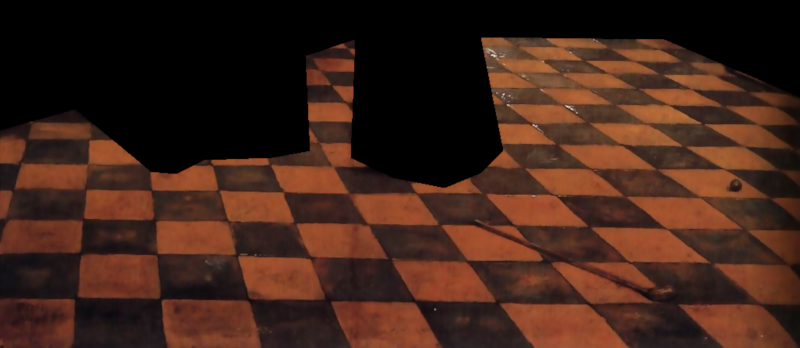
\includegraphics[scale=0.95]{bilateral2.png}};
			\node at (0, -3) {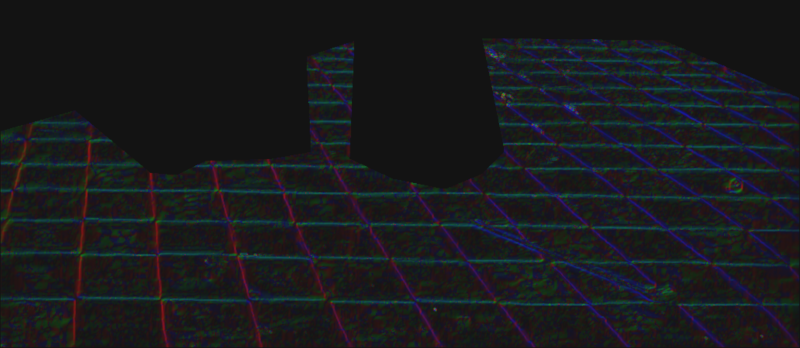
\includegraphics[scale=0.95]{sobel0.png}};
			\end{tikzpicture}
		\end{figure}
	\end{frame}

	\begin{frame}{Gradient (nettoyage)}
		\begin{figure}[h]
			\centering
			\begin{tikzpicture}[scale=0.8]
			\node (a) at (0, 0) {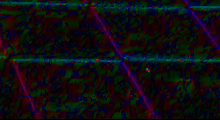
\includegraphics[scale=2.2]{sobel_wc.png}};
			\node (b) at (7.25, 0) {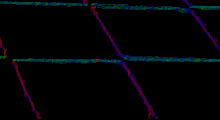
\includegraphics[scale=2.2]{sobel_c.png}};
			\draw[->, ultra thick] (a) -- node[above] {\small Nettoyage} (b);
			\node[align=center] (c) at (6, -2.2) {\footnotesize Effacé car la composante \\[-1mm]
				\footnotesize connexe est trop petite};
			\draw[->, thick, gray] (c.174) -- (0.98, -0.35);
			\node[align=center] (d) at (-0.3, -2.1) {\footnotesize Effacé car l'intensité \\[-1mm]
				\footnotesize est trop petite};
			\draw[->, thick, gray] (d.north) -- (-0.85, -0.5);
			\end{tikzpicture}
		\end{figure}
	\end{frame}

	\begin{frame}{Gradient (lissage)}
	\begin{algorithm}[H]
		\caption{Lissage de gradient}
		\begin{algorithmic}
			\State $M \gets \begin{bmatrix}
			0.0925 & 0.12 & 0.0925 \\
			0.12 & 0.15 & 0.12 \\
			0.0925 & 0.12 & 0.0925
			\end{bmatrix}$
			\Function{SmoothGrad}{$G, \Theta, x, y$}
			\State $a, b \gets 0, 0$
			\For{$i, j \in \{ -1, 0, 1 \}^2$}
			\State $coef \gets M[j+1][i+1] \times G[x+i][y+j]$
			\State $a \gets a + coef \times \cos \left( 2 \times \Theta[x+i][y+j] \right)$
			\State $b \gets b + coef \times \sin \left( 2 \times \Theta[x+i][y+j] \right)$
			\EndFor
			\State $\Theta[x][y] \gets \arg \left( a + ib \right) \, / \, 2$
			\EndFunction
		\end{algorithmic}
	\end{algorithm}
	\end{frame}

	\begin{frame}{Gradient (lissage)}
		\begin{figure}[h]
			\centering
			\begin{tikzpicture}
			\node[] (a) at (0, 0) {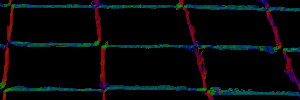
\includegraphics[scale=3.3]{sobel_ws.png}};
			\node[] (b) at (0, -3) {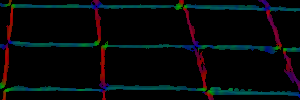
\includegraphics[scale=3.3]{sobel_s.png}};
			\node[below=3mm, white] at (a.150) {\small Sans lissage};
			\node[below=3mm, white] at (b.150) {\small Avec lissage};
			\end{tikzpicture}
		\end{figure}
	\end{frame}

	\begin{frame}{Gradient (nettoyage manuel)}
		\begin{figure}[h]
			\centering
			\begin{tikzpicture}
			\node (a) at (0, 0) {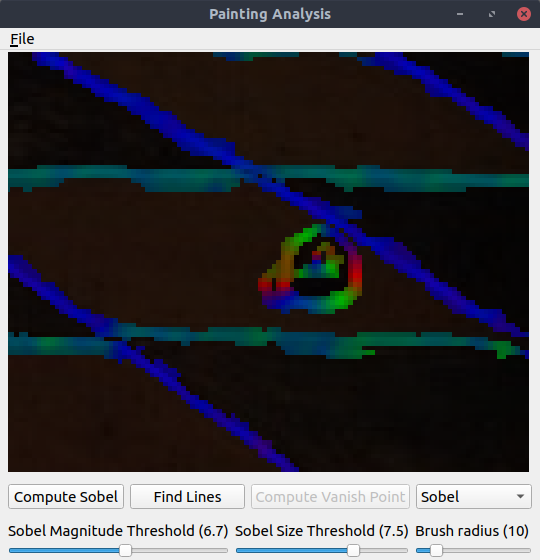
\includegraphics[scale=0.21]{w_man_c.png}};
			\node (b) at (6.6, 0) {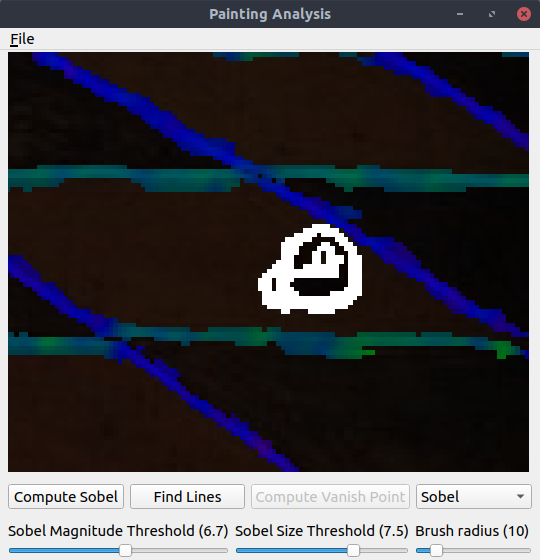
\includegraphics[scale=0.21]{man_c.png}};
			\draw[->, ultra thick] (a) -- node[above] {\small coup de brosse} (b);
			\end{tikzpicture}
		\end{figure}
	\end{frame}

	\begin{frame}{Transformée de Hough}
		\begin{figure}[h]
			\centering
			\begin{tikzpicture}[thick]
			\draw[red] (2.093, -0.9) -- node[below] {\small $1$} (1.57, -0.9)
						-- node[left] {\small $|a|$} (1.57, -0.1);
			\draw[green] (0.5, 0) arc(0:33.7:0.5) node[right, pos=0.7] {\small $\theta$};
			\draw[green] (0, 0) -- node[above] {\small $\rho$} (1.05, 0.7);
			\draw[->] (0, -1) -- node[right, pos=0.95] {\small $y$} (0, 3);
			\draw[->] (-1.5, 0) -- node[above, pos=0.95] {\small $x$} (3, 0);
			\draw[very thick, blue] (-0.5, 3) -- (2.17, -1);
			\node[red] at (0, 2.25) {$\bullet$};
			\node[red, right] at (0, 2.25) {\small $b$};
			\node at (5.8, 2.5) {$y = {\color{red} a} x + {\color{red} b} \quad \text{\color{red} \faThumbsODown}$};
			\node at (5.8, 1.5) {${\color{green} \rho} = x \cos {\color{green} \theta} + y \sin {\color{green} \theta} \quad \text{\color{green} \faThumbsOUp}$};
			\node at (5.8, 0.5) {${\color{green} \rho} \in \left[0; \, D\right] \quad {\color{green} \theta} \in \left[-\pi / 2; \, \pi\right]$};
			\end{tikzpicture}
		\end{figure}
	\end{frame}

\end{document}